\documentclass[10pt]{article}\usepackage[]{graphicx}\usepackage[]{color}
%% maxwidth is the original width if it is less than linewidth
%% otherwise use linewidth (to make sure the graphics do not exceed the margin)
\makeatletter
\def\maxwidth{ %
  \ifdim\Gin@nat@width>\linewidth
    \linewidth
  \else
    \Gin@nat@width
  \fi
}
\makeatother

\definecolor{fgcolor}{rgb}{0.345, 0.345, 0.345}
\newcommand{\hlnum}[1]{\textcolor[rgb]{0.686,0.059,0.569}{#1}}%
\newcommand{\hlstr}[1]{\textcolor[rgb]{0.192,0.494,0.8}{#1}}%
\newcommand{\hlcom}[1]{\textcolor[rgb]{0.678,0.584,0.686}{\textit{#1}}}%
\newcommand{\hlopt}[1]{\textcolor[rgb]{0,0,0}{#1}}%
\newcommand{\hlstd}[1]{\textcolor[rgb]{0.345,0.345,0.345}{#1}}%
\newcommand{\hlkwa}[1]{\textcolor[rgb]{0.161,0.373,0.58}{\textbf{#1}}}%
\newcommand{\hlkwb}[1]{\textcolor[rgb]{0.69,0.353,0.396}{#1}}%
\newcommand{\hlkwc}[1]{\textcolor[rgb]{0.333,0.667,0.333}{#1}}%
\newcommand{\hlkwd}[1]{\textcolor[rgb]{0.737,0.353,0.396}{\textbf{#1}}}%
\let\hlipl\hlkwb

\usepackage{framed}
\makeatletter
\newenvironment{kframe}{%
 \def\at@end@of@kframe{}%
 \ifinner\ifhmode%
  \def\at@end@of@kframe{\end{minipage}}%
  \begin{minipage}{\columnwidth}%
 \fi\fi%
 \def\FrameCommand##1{\hskip\@totalleftmargin \hskip-\fboxsep
 \colorbox{shadecolor}{##1}\hskip-\fboxsep
     % There is no \\@totalrightmargin, so:
     \hskip-\linewidth \hskip-\@totalleftmargin \hskip\columnwidth}%
 \MakeFramed {\advance\hsize-\width
   \@totalleftmargin\z@ \linewidth\hsize
   \@setminipage}}%
 {\par\unskip\endMakeFramed%
 \at@end@of@kframe}
\makeatother

\definecolor{shadecolor}{rgb}{.97, .97, .97}
\definecolor{messagecolor}{rgb}{0, 0, 0}
\definecolor{warningcolor}{rgb}{1, 0, 1}
\definecolor{errorcolor}{rgb}{1, 0, 0}
\newenvironment{knitrout}{}{} % an empty environment to be redefined in TeX

\usepackage{alltt}

\usepackage{amsmath,amssymb,amsthm}
\usepackage{fancyhdr,url,hyperref}
\usepackage{graphicx,xspace}
\usepackage{subfigure}
\usepackage{tikz}
\usetikzlibrary{arrows,decorations.pathmorphing,backgrounds,positioning,fit,through}

\oddsidemargin 0in  %0.5in
\topmargin     0in
\leftmargin    0in
\rightmargin   0in
\textheight    9in
\textwidth     6in %6in
%\headheight    0in
%\headsep       0in
%\footskip      0.5in

\newtheorem{thm}{Theorem}
\newtheorem{cor}[thm]{Corollary}
\newtheorem{obs}{Observation}
\newtheorem{lemma}{Lemma}
\newtheorem{claim}{Claim}
\newtheorem{definition}{Definition}
\newtheorem{question}{Question}
\newtheorem{answer}{Answer}
\newtheorem{problem}{Problem}
\newtheorem{solution}{Solution}
\newtheorem{conjecture}{Conjecture}

\pagestyle{fancy}

\lhead{\textsc{Prof. McNamara}}
\chead{\textsc{SDS/MTH 220: Lecture notes}}
\lfoot{}
\cfoot{}
%\cfoot{\thepage}
\rfoot{}
\renewcommand{\headrulewidth}{0.2pt}
\renewcommand{\footrulewidth}{0.0pt}

\newcommand{\shortans}{\vspace{1in}}
\newcommand{\mediumans}{\vspace{1.5in}}
\newcommand{\longans}{\vspace{2in}}

\newcommand{\ans}{\vspace{0.25in}}
\newcommand{\R}{{\sf R}\xspace}
\newcommand{\cmd}[1]{\texttt{#1}}

\rhead{\textsc{September 15, 2017}}
\IfFileExists{upquote.sty}{\usepackage{upquote}}{}
\begin{document}

\paragraph{Agenda}
\begin{enumerate}
  \itemsep0em
  \item Center, Shape, and Spread
\end{enumerate}

\paragraph{Warmup: Lurking Variables}

For each of the following pairs of variables, a statistically signficant positive relationship has been observed. Identify a potential lurking variable that might cause the spurious correlation.
\begin{enumerate}
  \itemsep0.5in
  \item The amount of ice cream sold in New England and the number of deaths by drowning
  \item The salary of U.S. ministers and the price of vodka
  \item The number of doctors in a region and the number of crimes committed in that region
  \item The number of storks sighted and the population of Oldenburg, Germany, over a six-year period
  \item The amount of coffee consumed and the prevalence of lung cancer
\end{enumerate}


\paragraph{IMDB movie data}
Today, we'll focus on data about movies. I've chosen to use a dataset available on Kaggle.com which includes information scraped from the Internet Movie Database (IMDB). \url{https://www.kaggle.com/deepmatrix/imdb-5000-movie-dataset/discussion}



\begin{knitrout}
\definecolor{shadecolor}{rgb}{0.969, 0.969, 0.969}\color{fgcolor}\begin{kframe}
\begin{alltt}
\hlkwd{library}\hlstd{(mosaic)}
\hlstd{movies} \hlkwb{<-} \hlkwd{read_csv}\hlstd{(}\hlstr{"http://www.science.smith.edu/~amcnamara/sds220/data/movies2.csv"}\hlstd{)}
\hlstd{movies} \hlopt
  \hlkwd{glimpse}\hlstd{()}
\end{alltt}
\begin{verbatim}
## Observations: 5,043
## Variables: 28
## $ color                     <chr> "Color", "Color", "Color", "Color", ...
## $ director_name             <chr> "James Cameron", "Gore Verbinski", "...
## $ num_critic_for_reviews    <int> 723, 302, 602, 813, NA, 462, 392, 32...
## $ duration                  <int> 178, 169, 148, 164, NA, 132, 156, 10...
## $ director_facebook_likes   <int> 0, 563, 0, 22000, 131, 475, 0, 15, 0...
## $ actor_3_facebook_likes    <int> 855, 1000, 161, 23000, NA, 530, 4000...
## $ actor_2_name              <chr> "Joel David Moore", "Orlando Bloom",...
## $ actor_1_facebook_likes    <int> 1000, 40000, 11000, 27000, 131, 640,...
## $ gross                     <int> 760505847, 309404152, 200074175, 448...
## $ genres                    <chr> "Action|Adventure|Fantasy|Sci-Fi", "...
## $ actor_1_name              <chr> "CCH Pounder", "Johnny Depp", "Chris...
## $ movie_title               <chr> "Avatar", "PiratesoftheCaribbeanAtWo...
## $ num_voted_users           <int> 886204, 471220, 275868, 1144337, 8, ...
## $ cast_total_facebook_likes <int> 4834, 48350, 11700, 106759, 143, 187...
## $ actor_3_name              <chr> "Wes Studi", "Jack Davenport", "Step...
## $ facenumber_in_poster      <int> 0, 0, 1, 0, 0, 1, 0, 1, 4, 3, 0, 0, ...
## $ plot_keywords             <chr> "avatar|future|marine|native|paraple...
## $ movie_imdb_link           <chr> "http://www.imdb.com/title/tt0499549...
## $ num_user_for_reviews      <int> 3054, 1238, 994, 2701, NA, 738, 1902...
## $ language                  <chr> "English", "English", "English", "En...
## $ country                   <chr> "USA", "USA", "UK", "USA", NA, "USA"...
## $ content_rating            <chr> "PG-13", "PG-13", "PG-13", "PG-13", ...
## $ budget                    <dbl> 237000000, 300000000, 245000000, 250...
## $ title_year                <int> 2009, 2007, 2015, 2012, NA, 2012, 20...
## $ actor_2_facebook_likes    <int> 936, 5000, 393, 23000, 12, 632, 1100...
## $ imdb_score                <dbl> 7.9, 7.1, 6.8, 8.5, 7.1, 6.6, 6.2, 7...
## $ aspect_ratio              <dbl> 1.78, 2.35, 2.35, 2.35, NA, 2.35, 2....
## $ movie_facebook_likes      <int> 33000, 0, 85000, 164000, 0, 24000, 0...
\end{verbatim}
\end{kframe}
\end{knitrout}

As the output suggests, the data has 5,043 observations (movies) and 28 variables. 

% \paragraph{Types of variables}
% We often break variables into two broad categories, categorical and quantitative. Categorical variables have only a few possible categories. A classic example is gender, which may have the categories ``male'', ``female'', and ``gender non-conforming.'' Quantitative variables (otherwise known as numeric variables) can have a larger range of options, including decimal numbers and integers. For example, consider age or height. 
% \\
% \\Which of the following variables would you categorize as quantitative? \hspace{0.1in} \verb#color#, \verb#duration#, \verb#director_facebook_likes#, \verb#facenumber_in_poster#, \verb#language#, \verb#content_rating#, \verb#imdb_score#.
% \ans

\paragraph{Thought Experiment}
Consider the following two variables:
\begin{itemize}
  \item The \verb#duration# of all the movies in the IMDB dataset. 
  \item The \verb#facenumber_in_poster# (number of faces detected in the movie poster). 
\end{itemize}

Think about the distribution of each variable, and discuss the following questions with a neighbor.
\begin{enumerate}
  \itemsep0.3in
  \item Draw the shape you believe each distribution has.  What features does it have? Is it symmetric? Is it normal? It is unimodal? [Make sure you label the axes on your distribution plot.] What is the range of each variable? 
  \mediumans
  \item How would you summarize each distribution numerically? Which measures are most appropriate?
  \item Suppose we added an additional face to each movie poster. How would the distribution of \verb#facenumber_in_poster# change? What would happen to your measures of center and spread? 
  \ans
\end{enumerate}

\paragraph{Describing Distributions}
We are going to hone in on the quantitative variables in this analysis, and start doing some EDA of their distributions. When describing distributions, three concepts are particularly useful: \emph{Center}, \emph{Shape}, and \emph{Spread}. 
\begin{itemize}
  \item Graphical techniques for summarizing the \emph{shape} of the distribution of one variable:
  \begin{itemize}
%    \item Stem (and leaf) plot [in R, {\tt stem()}]
    \item Histogram [\cmd{geom\_histogram()}]
    \item Density plot [\cmd{geom\_density()}]
    \item Box (and whisker) plot [\cmd{geom\_boxplot()}]
  \end{itemize}
  \item Numerical Techniques for summarizing the \emph{center} and \emph{spread} of the distribution of one variable:
  \begin{itemize}
    \item Center: mean [{\tt mean()}], median [{\tt median()}]
    \item Spread: standard deviation [{\tt sd()}], variance [{\tt var()}], range [{\tt range()}], IQR [{\tt IQR()}]
    \item (Center and spread can be seen together in {\tt favstats()})
  \end{itemize}
\end{itemize}

\paragraph{US box-office gross}
A box plot, histogram, and density plot reveal different features of the distribution of box-office gross. 
\begin{knitrout}
\definecolor{shadecolor}{rgb}{0.969, 0.969, 0.969}\color{fgcolor}\begin{kframe}
\begin{alltt}
\hlstd{movies} \hlkwb{<-} \hlstd{movies} \hlopt
  \hlkwd{filter}\hlstd{(country}\hlopt{==}\hlstr{"USA"}\hlstd{)}
\hlkwd{favstats}\hlstd{(}\hlopt{~}\hlstd{gross,} \hlkwc{data} \hlstd{= movies)}
\end{alltt}
\begin{verbatim}
##  min       Q1   median       Q3       max     mean       sd    n missing
##  703 10110274 32178777 72147000 760505847 55214607 71733124 3235     572
\end{verbatim}
\end{kframe}
\end{knitrout}


\begin{knitrout}
\definecolor{shadecolor}{rgb}{0.969, 0.969, 0.969}\color{fgcolor}\begin{kframe}
\begin{alltt}
\hlkwd{ggplot}\hlstd{(}\hlkwc{data}\hlstd{=movies,} \hlkwd{aes}\hlstd{(}\hlkwc{y}\hlstd{=gross,} \hlkwc{x}\hlstd{=}\hlnum{1}\hlstd{))} \hlopt{+} \hlkwd{geom_boxplot}\hlstd{()}
\hlkwd{ggplot}\hlstd{(}\hlkwc{data}\hlstd{=movies,} \hlkwd{aes}\hlstd{(}\hlkwc{x}\hlstd{=gross))} \hlopt{+} \hlkwd{geom_histogram}\hlstd{()}
\hlkwd{ggplot}\hlstd{(}\hlkwc{data}\hlstd{=movies,} \hlkwd{aes}\hlstd{(}\hlkwc{x}\hlstd{=gross))} \hlopt{+} \hlkwd{geom_density}\hlstd{()}
\end{alltt}
\end{kframe}
\end{knitrout}
\begin{knitrout}
\definecolor{shadecolor}{rgb}{0.969, 0.969, 0.969}\color{fgcolor}
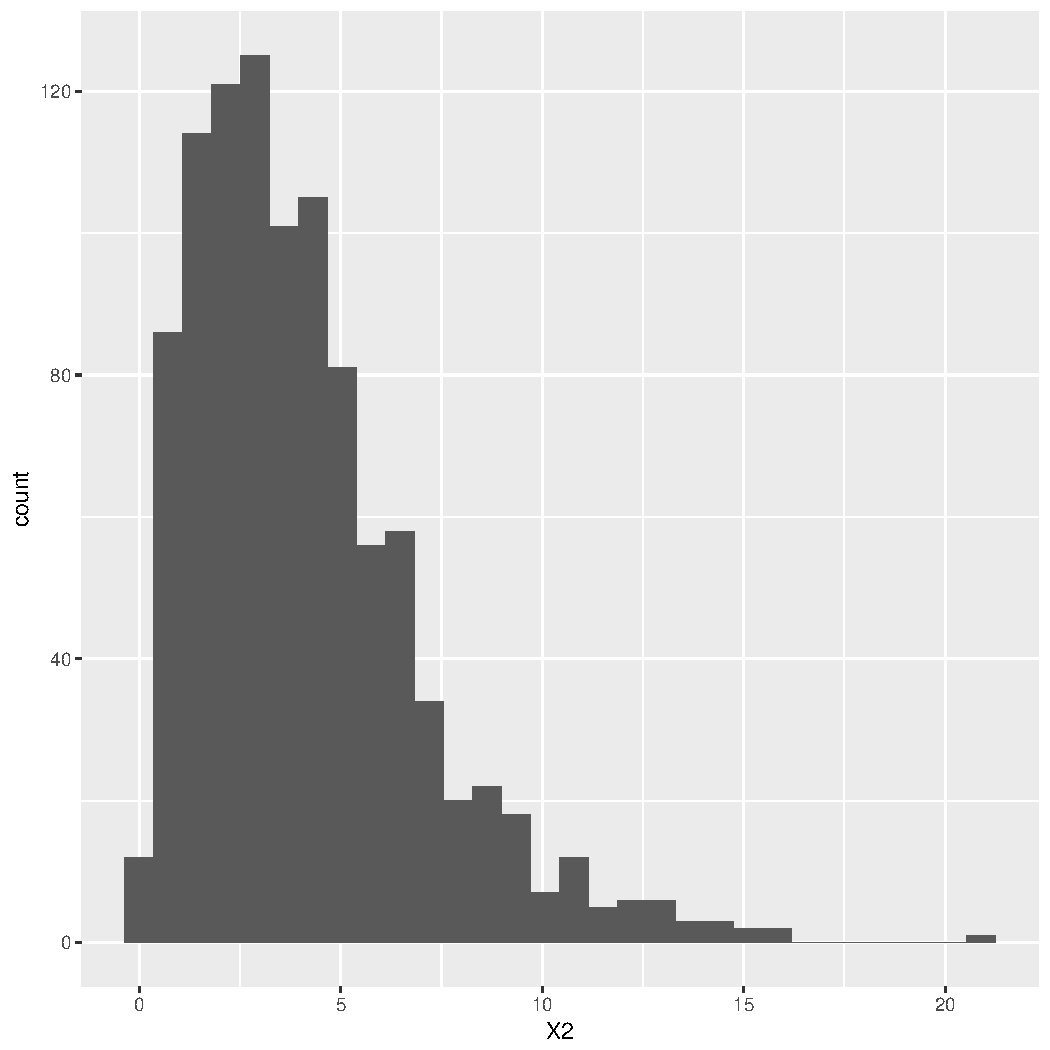
\includegraphics[width=\maxwidth]{figure/unnamed-chunk-5-1} 

\end{knitrout}

\begin{enumerate}
  \item Describe the distribution of box office gross using words. 
  \ans
  \item What information can you glean from the histogram or density plot that is not revealed by the numerical table or the box plot?
  \ans
  \item What information does the numerical table give you that is not available in the plots?
  \ans
  \ans
\end{enumerate}

% \paragraph{ggplot2}
% The graphs we have just seen were made using a graphics package for \verb#R# called \verb#ggplot2#. It maps variables in data to ``aesthetics'' (\verb#aes()#). The aesthetics can be used for a variety of geometric objects (like \verb#geom_histogram()#). RStudio has a great cheatsheet for \verb#ggplot2#, \url{https://www.rstudio.com/wp-content/uploads/2015/03/ggplot2-cheatsheet.pdf}
% 
% Thinking back to our question about \verb#duration# and \verb#facenumber_in_poster#, how would we write the code to check if our guesses about the distributions were correct? 
% \shortans

\paragraph{faceting} One great thing about \verb#ggplot2# is that it allows you to `facet' by another variable. (Essentially, make the same plot several times for different values of a second variable.) For example, maybe we think the distribution of \verb#gross# will be different depending on the \verb#content_rating#

\begin{knitrout}
\definecolor{shadecolor}{rgb}{0.969, 0.969, 0.969}\color{fgcolor}\begin{kframe}
\begin{alltt}
\hlstd{movies} \hlkwb{<-} \hlstd{movies} \hlopt
  \hlkwd{filter}\hlstd{(content_rating} \hlopt \hlkwd{c}\hlstd{(}\hlstr{"PG"}\hlstd{,} \hlstr{"PG-13"}\hlstd{,} \hlstr{"R"}\hlstd{))}
\hlkwd{ggplot}\hlstd{(}\hlkwc{data}\hlstd{=movies,} \hlkwd{aes}\hlstd{(}\hlkwc{x}\hlstd{=gross))} \hlopt{+} \hlkwd{geom_histogram}\hlstd{()} \hlopt{+} \hlkwd{facet_grid}\hlstd{(}\hlopt{~}\hlstd{content_rating)}
\end{alltt}
\end{kframe}
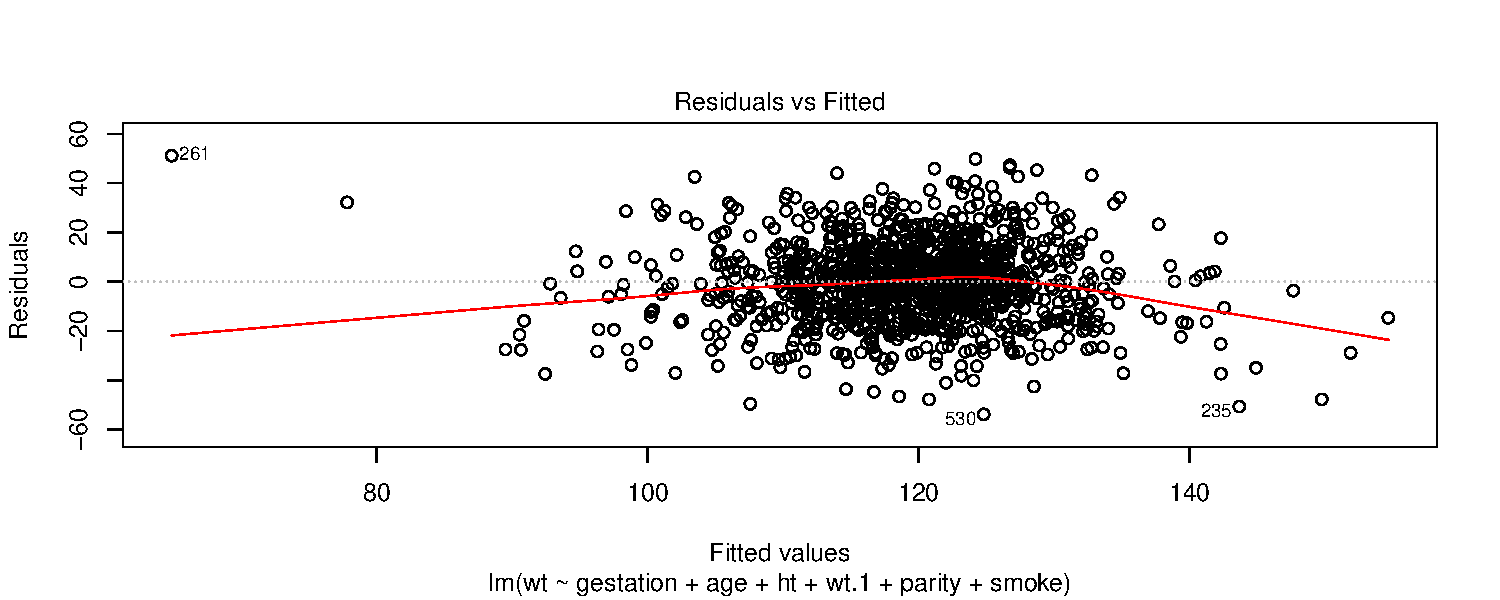
\includegraphics[width=\maxwidth]{figure/unnamed-chunk-6-1} 

\end{knitrout}

\paragraph{Relationships}
With a partner, brainstorm some relationships you think might exist in the data. What distributions of quantitative variables likely look different depending on the value of another categorical variable? 



% \newpage
% %'
% \subsection*{Instructor's Notes}
% %'
% \url{http://en.wikipedia.org/wiki/Household_income_in_the_United_States#Household_income}
% %'



\end{document}
